\chapter{\textit{If e else}}
\section*{Introdução}
    Neste capítulo aprofundaremos nosso estudo de programação por meio de comandos que permitem a tomada de decisão, ou seja,  estruturas auxiliares que estabelecem uma condição para a execução de um comando principal. \textsl{Ficou confuso? Não se preocupe, vou explicar a seguir!}

\section{Estruturas de decisão}
    Desde o momento em que acordamos, estamos tomando decisões, às vezes até sem perceber! Por exemplo, optar por ficar alguns minutos a mais na cama e adiar o despertador ou decidir levantar no instante em que ele tocar. Vamos supor que amanhã você tem uma prova muito importante às 8 horas da manhã, o fato de escolher ignorar o despertador e dormir mais pode resultar em consequências, como perder aquela prova de final de semestre e, possivelmente, acabar ficando com nota baixa. Como não é isso que queremos, é sempre bom acordar cedo em dias que tivermos provas pela manhã.
    
    \begin{center}
        \textsl{Estabelecemos uma condição para acordar cedo, você percebeu? A condição de acordar cedo é se houver uma prova pela manhã... É exatamente isso que faremos neste capítulo! Estabeleceremos condições para que o \textsl{Sparki} realize determinada ação!}
    \end{center}
   
    \indent As estruturas de decisão que utilizaremos são ``if'' e ``else'', elas significam ``se'' e ``senão'' em inglês, respectivamente.
    
\section{Como utilizar ``if'' e else''?}
    A seguir temos exemplos de uso dessas estruturas:
    \\
    \\
    \textsc{Exemplo 1)} Exemplo base. (Apenas para fins didáticos)
    \\
    \\
    \noindent \mintinline{cpp}{if}(Condição 1) \{\\
    \indent Ação 1;\\
    \} \mintinline{cpp}{else} \{\\
    \indent Ação 2;\\
    \}\\
    
    Esse exemplo significa que, se a ``Condição 1'' for verdadeira, o Sparki\textsl{Sparki} executará a ``Ação 1'', senão, ele executará a ``Ação 2''. Utilizar o \mintinline{cpp}{else} como uma opção alternativa ao \mintinline{cpp}{if()} é optativo, ou seja, podem existir expressões condicionais apenas com \mintinline{cpp}{if()}.
    
    \begin{center}
    {\large{Reflita}}: A ``Ação 1'' e a ``Ação 2'' poderiam ser executadas sequencialmente, em apenas uma leitura desse código ?
    \end{center}
    
    A seguir temos uma tabela com todas as opções de execução do código desse primeiro exemplo: (Tente entender a tabela, apenas decorar pode te deixar confuso mais para frente)
    
    \begin{center}
    \begin{tabular}{|c|c|c|}
    \hline
    Condição 1 & Ação 1 & Ação 2 \\ \hline
    Verdadeira & Executa & Não executa \\ \hline
    Falsa & Não executa & Executa \\ \hline
    \end{tabular}
    \end{center}
    
    \textsc{Exemplo 2)} Exemplo da explicação. (Apenas para fins didáticos)
    \\
    \\
    \noindent \mintinline{cpp}{if}(For dia de prova) \{\\
    \indent Acordar mais cedo;\\
    \} \mintinline{cpp}{else} \{\\
    \indent Acordar no horário normal;\\
    \}\\
    
    Neste caso, se for o dia da prova, devemos acordar mais cedo e, se não for o dia da prova, devemos acordar no horário normal. A segunda ação apenas ocorre se a primeira não ocorrer, logo, essas duas ações não poderiam ser executadas sequencialmente, ou seja, em uma mesma verificação da condição de ser ou não dia de prova.\\
    
    \textsc{Exemplo 3)} Exemplo com ``else if''. (Apenas para fins didáticos)
    \\
    \\
    \noindent \mintinline{cpp}{if}(Condição 1) \{\\
    \indent Ação 1;\\
    \} \mintinline{cpp}{else if}(Condição 2) \{ \\
    \indent Ação 2;\\
    \} \mintinline{cpp}{else} \{\\
    \indent Ação 3;\\
    \}\\
    
    \textit{Agora apareceram \mintinline{cpp}{else} e \mintinline{cpp}{if} em uma mesma linha, o que isso significa?} \\
    Para entender os dois termos juntos, vamos revisar o significado deles separados. \mintinline{cpp}{else} significa: ``se as condições anteriores forem falsas, executar o comando dentro das chaves''. \mintinline{cpp}{if()} significa: ``se a condição dentro dos parênteses for verdadeira, executar o comando dentro das chaves''. Consequentemente, a expressão \mintinline{cpp}{else if()} implica na execução do comando apenas se as condições anteriores forem falsas e a condição dentro do parênteses for verdadeira.
    
    \begin{center}
    \begin{tabular}{|c|c|c|c|c|}
    \hline
    Condição 1 & Ação 1 & Condição 2 & Ação 2 & Ação 3\\ \hline
    Verdadeira & Executa & Falsa & Não executa & Não executa \\ \hline
    Verdadeira & Executa & Verdadeira & Não executa & Não executa \\ \hline
    Falsa & Não executa & Verdadeira & Executa & Não executa \\ \hline
    Falsa & Não executa & Falsa & Não executa & Executa \\ \hline
    \end{tabular}
    \end{center}
    
    \textsc{Exemplo 4)} Imagine uma situação hipotética em que existam 3 compromissos na sua agenda, no mesmo dia e horário, e você terá que escolher apenas um, de acordo com a previsão do tempo. (Apenas para fins didáticos)
    \\
    \\
    \noindent \mintinline{cpp}{if}(Estiver fazendo muito calor) \{ \\
    \indent Ir ao clube; \\
    \} \mintinline{cpp}{else if}(Estiver chovendo) \{ \\
    \indent Ver um filme em casa;\\
    \} \mintinline{cpp}{else if}(Estiver nevando) \{ \\
    \indent Ir esquiar;\\
    \} \mintinline{cpp}{else} \{ \\
    \indent Ir ao cinema.\\
    \}\\
    
    \textit{Isshh... Agora ficou complicado! E se a previsão do tempo afirmar que vai chover e nevar nesse dia? Qual compromisso eu escolho?} 
    \\
    Essa é fácil! É necessário apenas observar qual das condições será lida primeiro nesse código, ou seja, o que vier primeiro! Como a condição ``Estiver chovendo'' aparece primeiro, o compromisso seria ``Ver um filme em casa''.
    
    \textit{E qual seria a condição para ``Ir ao cinema''?} 
    \\
    A condição seria a negação das anteriores, neste caso, se não estivesse fazendo muito calor, nem chovendo, nem nevando.
    
    Uma curiosidade dessa estrutura condicional é que se escrevermos ``1'' dentro dos parênteses do \mintinline{cpp}{if()}, ele será verdadeiro e o que estiver dentro das chaves será executado. Assim, se escrevermos ``0'' dentro dos parênteses, o \mintinline{cpp}{if()} será falso e o que estiver dentro das chaves não será executado. Isso se dá porque a programação possui uma base binária, ou seja, ela é baseada em vários ``1'' e ``0''.
    
    \section{Operações de comparação}
    
    Iremos aprender nesta seção os tipos de operadores que podemos utilizar para comparar dois valores ou incógnitas. Lembrando que eles devem ser utilizados apenas dentro do parênteses do \mintinline{cpp}{if()}. São eles:
    
    \begin{itemize}
        \item ``=='' para verificar se os dois valores são iguais.
        \item ``!='' para verificar se os dois valores são diferentes.
        \item ``>'' para verificar se o primeiro é maior que o segundo.
        \item ``>='' para verificar se o primeiro é maior que o segundo ou igual a ele.
        \item ``<'' para verificar se o primeiro é menor que o segundo.
        \item ``<='' para verificar se o primeiro é menor que o segundo ou igual a ele.
    \end{itemize}
    
    Agora que você já entendeu como funcionam as expressões condicionais e os operadores de comparação, vamos para um exemplo de verdade!
    \\
    \\
    \textsc{Exemplo 1)} Atribuiremos o valor 2042385 à variável x e queremos que o \textsl{Sparki} responda se esse número é ímpar ou par. Para isso, utilizaremos a informação da sessão anterior sobre os ``1'' e os ``0''.
    
    \begin{minted}{cpp}
    #include <Sparki.h>
    void setup()
    {
    }
    void loop()
    {
        int x = 2042385;
        sparki.clearLCD();
        if(x % 2) {
            sparki.print("O numero e impar.");
        } else {
            sparki.print("O numero e par.");
        }
        sparki.updateLCD();
        delay(1000);
    }
    \end{minted}
    
    Sabemos que o número 2042385 é ímpar pela regra da divisão por 2, que afirma que um número é divisível por 2 quando o último algarismo dele for divisível por 2. Nesse código, não utilizamos essa regrinha, mas sim o método mais tradicional, fazemos o \textsl{Sparki} verificar se a divisão desse número por 2 é exata, ou seja, se o resto é 0. Assim, o \textsl{Sparki} chega a mesma conclusão que chegamos, que o número 2042381 é ímpar, e imprime essa informação no LCD.
    
    \begin{center}
    \textcolor{teal}{Lembrando:}
    O símbolo ``\%'' significa o resto da divisão do primeiro número pelo segundo.
    \end{center}
    
    \textsc{Exemplo 2)} Dessa vez, faremos com que o \textsl{Sparki} responda se o número 2042385 é divisível por 3 e por 5.
    
    \begin{minted}{cpp}
    #include <Sparki.h>
    void setup()
    {
    }
    void loop()
    {
        int x = 2042385;
        sparki.clearLCD();
        if((x % 3) == 0) {
            sparki.println("O numero e divisivel por 3.");
        } else {
            sparki.println("O numero nao e divisivel por 3.");
        }
        if((x % 5) == 0) {
            sparki.print("O numero e divisivel por 5.");
        } else {
            sparki.print("O numero nao e divisivel por 5.");
        }
        sparki.updateLCD();
        delay(1000);
    }
    \end{minted}
    
    Esse exemplo é parecido com o anterior, mas ele está aqui para mostrar que podemos inserir duas estruturas condicionais independentes em um mesmo código. As duas comparações para saber se o número é divisível por 3 e por 5 não dependem uma da outra, pois um número pode ser divisível por 3 e por 5 ao mesmo tempo, por isso que existem dois \mintinline{cpp}{if()} e dois \mintinline{cpp}{else}. Consequentemente, o \textsl{Sparki} imprimirá duas mensagens na tela, na primeira linha: ``O numero e divisivel por 3'' e na segunda: ``O numero e divisivel por 5''.
    
    \textsc{Exemplo 3)} Exemplo de comparação de variáveis.
    
    \begin{minted}{cpp}
    #include <Sparki.h>
    void setup()
    {
    }
    void loop()
    {
        int x = 10;
        int y = 100;
        sparki.clearLCD();
        if(x >= y) {
            sparki.print("Condicao 1");
        } else if(y != (x * x)) {
            sparki.print("Condicao 2");
        } else if((y / x) >= x) {
            sparki.print("Condicao 3");
        } else if((y - 100) <= x){
            sparki.print("Condicao 4");
        }
        sparki.updateLCD();
        delay(1000);
    }
    \end{minted}
    
    Então, já sabe o que o \textsl{Sparki} fará ao ler este código? Vamos ver passo a passo:
    
    \begin{itemize}
        \item[Condição 1)]
        \begin{eqnarray}
        x & == & y\\
        10 & == & 100 \nonumber     \end{eqnarray}
        Essa afirmação é FALSA, logo, o \textsl{Sparki} não executará a ação entre as chaves.
        \item[Condição 2)]
        \begin{eqnarray}
        y & != & (x * x)\\
        100 & != & 10 * 10 \nonumber\\
        100 & != & 100 \nonumber
        \end{eqnarray}
        Essa afirmação também é FALSA, por isso a ação não será executada.
        \item[Condição 3)]
        \begin{eqnarray}
        (y / x) & >= & x\\
        (100 / 10) & >= & 10 \nonumber\\
        10 & >= & 10 \nonumber\\
        \end{eqnarray}
        Essa afirmação é verdadeira, logo, o \textsl{Sparki} executará a ação entre as chaves, imprimirá no LCD ``Condicao 3''.
        \item[Condição 4)]
        Essa condição não será nem lida, pois ela só poderia ser executada se todos os \mintinline{cpp}{if()} anteriores, dentro dessa estrutura condicional, fossem falsos.
    \end{itemize}
    
    \begin{center}
    \textcolor{teal}{Lembrando:}
    Sempre devemos executar a operação dentro dos parênteses antes dos operadores de comparação.
    \end{center}

\section{Fluxograma ou Diagrama de Fluxo}

    \begin{center}
    \textbf{Definição} 
    \\
    Uma representação gráfica de passos sequenciais e decisões a serem tomadas durante a execução de um processo.
    \end{center}
    
    Esboçar um Fluxograma antes de programar pode ser muito útil, principalmente quando se está aprendendo ainda. Dentre as principais vantagens de se fazer um Fluxograma, temos:
    \begin{itemize}
        \item Poder escolher a melhor solução para o problema;
        \item Organizar as ideias antes de começar a programar de fato;
        \item Evitar erros de lógica.
    \end{itemize}

    Por ser um representação gráfica de um programa, iremos aprender símbolos para cada tipo de execução, como, por exemplo, o início e o fim do programa, as entradas de informação, as ações do \textsl{Sparki}, as tomadas de decisão e o fluxo de informações. A figura a seguir mostra os símbolos gráficos correspondentes a cada um dos exemplos citados:
    
    \begin{figure}[h]
    \caption{Símbolos de um Fluxograma.}
     
    \centering 
    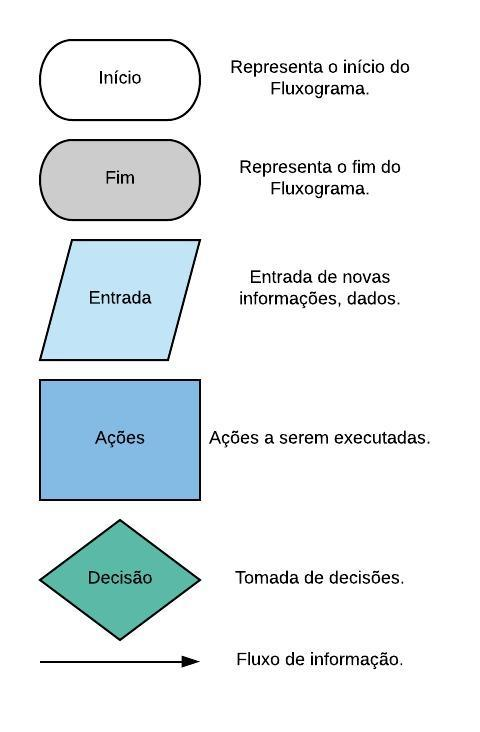
\includegraphics[width=5cm]{Figuras/Diagrama em branco.jpeg}
    \label{figura:Diagrama em branco.jpeg}
    \end{figure}
 
\section{Operadores lógicos}
    Nesta seção, iremos aprender a lidar com comparações que envolvem mais de um fator a ser analisado e, para isso, utilizaremos o início da teoria da Álgebra Booleana, criada por George Boole. 
 
     Na Álgebra de Boole, existem 3 tipos de operadores lógicos: E, OU e NÃO, cada um com uma funcionalidade própria. Eles devem ser usados dentro de condicionais \mintinline{cpp}{if()} para ligar duas comparações ou para negar uma ou mais comparações.
 
\subsection{E (AND)}
 
    Este operador depende de pelo menos dois ``resultados'' de afirmações, por exemplo, vamos supor que você quer ir à piscina, mas você apenas irá se estiver fazendo sol \textbf{E} se a piscina estiver limpa. Então, a 1ª afirmação é: se estiver fazendo sol e a 2ª afirmação é: se a piscina estiver limpa. O operador AND vai funcionar como uma ``ponte'' de ligação entre essas duas afirmações. 
    
    \begin{center}
        A condição estabelecida pelo \mintinline{cpp}{if()}, com o AND entre as afirmações, será VERDADEIRA apenas quando as afirmações forem ambas VERDADEIRAS.
    \end{center}
    
    \textit{Então o AND vai ser uma comparação entre duas comparações?? Que confuso!}
    
    Mais ou menos... É mais certo dizer que o AND irá realizar uma operação entre as duas comparações/afirmações. Utilizando o exemplo anterior, as duas afirmações têm que ser verdadeiras, ou seja, 1) tem que estar fazendo sol e 2) a piscina tem que estar limpa para que a comparação seja verdadeira e você possa ir à piscina.
    \\
    \\
    \textsc{Exemplo 0)} Exemplo da explicação, apenas para fins didáticos.
    \\
    \\
    \mintinline{cpp}{if}(Fizer sol AND Piscina estiver limpa) \{\\
    \indent Ir à piscina;\\
    \} \mintinline{cpp}{else} \{\\
    \indent Não ir à piscina;\\
    \}
    
    Se a comparação 1 der VERDADEIRA e a comparação 2 der FALSA, o \mintinline{cpp}{if()} não será realizado e você não irá à piscina. Porém, se as duas comparações derem VERDADEIRAS, o \mintinline{cpp}{if()} será realizado e você poderá ir à piscina.
    
    Agora, vamos fazer um esquema com todas as possibilidades de combinação entre duas comparações e ver o resultado final:
    
    \begin{itemize}
        \item VERDADEIRO AND VERDADEIRO -> Resultado: VERDADEIRO
        \item VERDADEIRO AND FALSO -> Resultado: FALSO
        \item FALSO AND VERDADEIRO -> Resultado: FALSO
        \item FALSO AND FALSO -> Resultado: FALSO
    \end{itemize}
    
    \begin{center}
    \textcolor{teal}{Lembrando:}
    Resultado: VERDADEIRO, significa que o \mintinline{cpp}{if()} será executado. 
    Resultado: FALSO, significa que o \mintinline{cpp}{if()} não será executado.
    \end{center}
 
    \textit{Tá, mas como eu aplico isso na programação?}
        
    Na programação, utilizamos os caracteres ``\&\&'' para simbolizar o AND. Aqui temos um exemplo:
    \\
    \\
    \textsc{Exemplo 1)} Neste exemplo, serão criadas 3 variáveis para armazenar a idade de 3 crianças: o Enzo, que tem 1 ano, a Valentina, que tem 2 anos, e a Sofia com 3 anos. Se a idade das 3 crianças forem iguais, o \textsl{Sparki} andará para frente, se a Sofia for a mais velha e o Enzo o mais novo, o \textsl{Sparki} andará para trás, e, por último, se as duas condições anteriores forem falsas, o \textsl{Sparki} ficará parado.

    \begin{minted}{cpp}
    #include <Sparki.h>
    void setup()
    {
    }
    void loop()
    {
        int idade_enzo = 1;
        int idade_valentina = 2;
        int idade_sofia = 3;
        if(idade_enzo == idade_valentina && idade_enzo != idade_sofia){
            //Se o Enzo e a Valentina tiverem a mesma idade e a Sofia tiver uma idade diferente
            //Neste caso, FALSO AND VERDADEIRO -> Resultado: FALSO
            sparki.moveForward();
        } else if(idade_valentina > idade_enzo && idade_sofia > idade_valentina) {
            //Se o primeiro caso for falso e a Sofia for mais velha que a Valentina, que for mais velha que o Enzo
            //Neste caso, VERDADEIRO AND VERDADEIRO -> Resultado: VERDADEIRO
            sparki.moveBackward();
        } else {
            //Se o primeiro e o segundo caso forem falsos
        }
    }
    \end{minted}
    
    O \textsl{Sparki} andará para trás.
    \begin{itemize}
        \item[Condição 1)]
        \begin{eqnarray}
        idade\_enzo & = & idade\_valentina\\
        1 & = & 2 \nonumber     \end{eqnarray}
        Essa afirmação é FALSA.
        \begin{eqnarray}
        idade\_enzo & != & idade\_sofia\\
        1 & != & 3 \nonumber
        \end{eqnarray}
        Essa afirmação é VERDADEIRA.
        Como temos o ``\&\&'' (AND) ligando as duas afirmações, a comparação será FALSA.
        \item[Condição 2)]
        \begin{eqnarray}
        idade\_valentina & > & idade\_enzo
        \end{eqnarray}
        Essa afirmação é VERDADEIRA.
        \begin{eqnarray}
        idade\_sofia & > & idade\_valentina
        \end{eqnarray}
        Essa afirmação também é VERDADEIRA. Como as duas afirmações são verdadeiras e o ``\&\&'' (AND) está ligando-as, a comparação será VERDADEIRA.
    \end{itemize} 
    
    \textsc{Exemplo 2)} Um exemplo com as mesmas variáveis anteriores, mas um pouco mais complicado.
    
    \begin{minted}{cpp}
    #include <Sparki.h>
    void setup()
    {
    }
    void loop()
    {
        int idade_enzo = 1;
        int idade_valentina = 2;
        int idade_sofia = 3;
        sparki.clearLCD();
        if((idade_sofia - idade_valentina) == idade_enzo && (idade_valentina - idade_enzo) == 3) {
            //VERDADEIRO AND FALSO -> Resultado: FALSO
            sparki.drawCircleFilled(63, 32, 10);
        } else if((idade_enzo + 1) != 2 && (idade_valentina - idade_enzo) != idade_sofia) {
            //FALSO AND VERDADEIRO -> Resultado: FALSO
            sparki.drawRectFilled(10,0, 15, 30);
        } else if((idade_enzo * 6) == (idade_valentina * 3)) {
            //VERDADEIRO
            sparki.drawChar(10, 1, 'a');
        } else {
            sparki.drawString(40, 4, "123");
        } 
        sparki.updateLCD();
        delay(1000);
    }
    \end{minted}
    
    O \textsl{Sparki} irá imprimir o caracter ``a'' no LCD.
    \begin{itemize}
        \item[Condição 1)]
        \begin{eqnarray}
        (idade\_sofia - idade\_valentina) & = & idade\_enzo\\
        (3 - 2) & = & 1 \nonumber \\
        1 & = & 1 \nonumber
        \end{eqnarray}
        Essa afirmação é VERDADEIRA.
        \begin{eqnarray}
        (idade\_valentina - idade\_enzo) & = & 3\\
        (2 - 1) & = & 3 \nonumber \\
        1 & = & 3 \nonumber
        \end{eqnarray}
        Essa afirmação é FALSA.
        Como temos o ``\&\&'' (AND) ligando essas duas afirmações, a comparação será FALSA.
        \item[Condição 2)] 
        \begin{eqnarray}
        (idade\_enzo + 1) & != & 2\\
        (1 + 1) & != & 2 \nonumber \\
        2 & != & 2 \nonumber
        \end{eqnarray}
        Essa afirmação é FALSA.
        \begin{eqnarray}
        (idade\_valentina - idade\_enzo) & != & idade\_sofia)\\
        (2 - 1) & != & 3 \nonumber \\
        1 & != & 3 \nonumber
        \end{eqnarray}
        Essa afirmação é VERDADEIRA. Como o ``\&\&'' (AND) está ligando essas duas afirmações, a comparação será FALSA
        \item[Condição 3)] 
        \begin{eqnarray}
        (idade\_enzo * 6) & = & (idade\_valentina * 3)\\
        (1 * 6) & = & (2 * 3) \nonumber \\
        6 & = & 6 \nonumber 
        \end{eqnarray}
        Essa afirmação é VERDADEIRA, logo, a comparação também é.
    \end{itemize}
    
    \begin{center}
    \textcolor{cyan}{Para não esquecer!}
    \\``And'' traduzido para o português significa ``e''.
    \end{center}
     
\subsection{OU (OR)}
    Este operador deve ser colocado entre duas ou mais afirmações, assim como o AND. Vamos supor que a sua mãe está viajando e você combinou de se encontrar com ela quando ela chegasse no aeroporto. O combinado foi o seguinte: ela mandaria mensagem \textbf{OU} ligaria quando estivesse embarcando no voo de volta, e você sairia de casa por volta de 30 minutos depois, para se encontrar com ela no aeroporto.
    
    \begin{center}
        A condição estabelecida pelo \mintinline{cpp}{if()}, com o OR entre as afirmações, será VERDADEIRA se pelo menos uma das duas comparações forem VERDADEIRAS.
    \end{center}
   
    \textsc{Exemplo 0)} Exemplo da explicação, apenas para fins didáticos.
    \\
    \\
    \mintinline{cpp}{if}(Sua mãe te mandasse mensagem OR Sua mãe te ligasse) \{\\
    \indent Esperar 30 minutos;\\
    \indent Sair de casa;\\
    \} \mintinline{cpp}{else} \{\\
    \indent Continuar esperando a mensagem ou a ligação;\\
    \}
     
     Então, se a sua mãe te ligasse (afirmação VERDADEIRA) mas não te mandasse mensagem (afirmação FALSA), a condição do \mintinline{cpp}{if()} seria VERDADEIRA e você esperaria 30 minutos para sair de casa. Se as duas afirmações foram VERDADEIRAS, ou seja, se ela te mandar mensagem e te ligar, a condição \mintinline{cpp}{if()} também será VERDADEIRA, neste caso, você também executará as ações dentro das chaves do \mintinline{cpp}{if()}.
     A seguir temos todos os resultados possíveis para um OR entre duas afirmações:
     
     \begin{itemize}
        \item VERDADEIRO OR VERDADEIRO -> Resultado: VERDADEIRO
        \item VERDADEIRO OR FALSO -> Resultado: VERDADEIRO
        \item FALSO OR VERDADEIRO -> Resultado: VERDADEIRO
        \item FALSO OR FALSO -> Resultado: FALSO
    \end{itemize}
    
    Na programação, utilizamos os caracteres ``||'' para simbolizar o OR.
    \\
    \\
    
    \textsc{Exemplo 1)}
     
     \begin{minted}{cpp}
    #include <Sparki.h>
    void setup()
    {
    }
    void loop()
    {
        int idade_enzo = 1;
        int idade_valentina = 2;
        int idade_sofia = 3;
        if(idade_enzo == idade_valentina || idade_sofia != idade_ valentina) {
        //Neste caso, FALSO OR VERDADEIRO -> Resultado: VERDADEIRO
        sparki.moveBackward();
        } else if(idade_valentina ==  (idade_sofia - 1) || (idade_valentina + 1) == idade_sofia) {
        //Neste caso, VERDADEIRO OR VERDADEIRO -> Resultado: VERDADEIRO
        sparki.moveForward();
        } else {
        //Se a primeira e a segunda condição forem falsas
        sparki.moveRight();
        }
    }
    \end{minted}
    
    O \textsl{Sparki} andará para trás.
    \begin{itemize}
        \item[Condição 1)] 
        \begin{eqnarray}
        idade\_enzo & = & idade\_valentina
        \end{eqnarray}
        Essa afirmação é FALSA.
        \begin{eqnarray}
        idade\_sofia & != & idade\_valentina
        \end{eqnarray}
        Essa afirmação é VERDADEIRA. Como o ``||'' (OR) liga essas duas afirmações, sabemos que a comparação será VERDADEIRA.
        \item[Condição 2)] Essa condição não será nem lida, pois ela só poderia ser executada se todos os \mintinline{cpp}{if()} anteriores, dentro dessa estrutura condicional, fossem falsos.
    \end{itemize}

    \textsc{Exemplo 2)}
     
    \begin{minted}{cpp}
    #include <Sparki.h>
    void setup()
    {
    }
    void loop()
    {
        int idade_enzo = 1;
        int idade_valentina = 2;
        int idade_sofia = 3;
        sparki.clearLCD();
        if(idade_valentina != 2 || idade_enzo != 1) {
            //FALSO OR FALSO -> Resultado: FALSO
            sparki.print("Condicao 1");
        } else if(idade_sofia != (idade_valentina - 1) || idade_sofia == idade_enzo) {
            //VERDADEIRO OR FALSO -> Resultado: FALSO
            sparki.print("Condicao 2");
        } else if((idade_enzo + 2) == (idade_sofia + 1) ||     idade_enzo == (4 - idade_sofia)) {
            //FALSO OR VERDADEIRO -> Resultado: FALSO
            sparki.print("Condicao 3");
        } else {
            sparki.print("Nenhuma das anteriores");
        }
        sparki.updateLCD();
        delay(1000);
    }
    \end{minted}
    
    O \textsl{Sparki} irá imprimir na tela ``Nenhuma das anteriores''.
    \begin{itemize}
        \item[Condição 1)] 
        \begin{eqnarray}
        idade\_valentina != 2\\
        idade\_enzo != 1 \nonumber
        \end{eqnarray}
        Essa afirmação é FALSA.
        \item[Condição 2)]
        \begin{eqnarray}
        idade\_sofia & = & idade\_enzo;
        \end{eqnarray}
        Essa afirmação é FALSA.
        \item[Condição 3)]
        \begin{eqnarray}
        (idade\_enzo + 2) & = & (idade\_sofia + 1)\\
        (1 + 2) & = & (3 + 1) \nonumber \\
        3 & = & 4 \nonumber
        \end{eqnarray}
        Essa afirmação é FALSA.
    \end{itemize}
     
    \begin{center}
        \textcolor{cyan}{Para não esquecer!}
        \\``Or'' traduzido para o português significa ``ou''.
    \end{center}
     
\subsection{NÃO (NOT)}

    \begin{itemize}
        \item NOT(VERDADEIRO) -> Resultado: FALSO
        \item NOT(FALSO) -> Resultado: VERDADEIRO
    \end{itemize}
    
    Na programação, utilizamos o caracter ``!'' para simbolizar o NOT.
    \\
    \\
     \textsc{Exemplo 1)}
     
     \begin{minted}{cpp}
    #include <Sparki.h>
    void setup()
    {
    }
    void loop()
    {
        int idade_enzo = 1;
        int idade_valentina = 2;
        int idade_sofia = 3;
        if(!(idade_enzo == 1) {
            //NOT(VERDADEIRO) -> Resultado: FALSO
        } else if(!(idade_valentina == 3)) {
            //NOT(FALSO) -> Resultado: VERDADEIRO
            sparki.moveForward();
        } else if(!(idade_sofia != 3)) {
            //NOT(FALSO) -> Resultado: VERDADEIRO
            sparki.moveBackward();
        }
    }
    \end{minted}
    
    O \textsl{Sparki} andará para frente, pois
    \begin{itemize}
        \item[Condição 1)]
        \begin{eqnarray}
        !(idade\_enzo & = & 1)\\
        !(1 & = & 1) \nonumber         \end{eqnarray}
        Sabemos que a afirmação 1 = 1 é VERDADEIRA, mas há um caracter ``!'' antes dela, por isso, ela acaba se tornando FALSA.
        \item[Condição 2)]
        \begin{eqnarray}
        !(idade\_valentina & = & 3)\\
        !(2 & = & 3) \nonumber
        \end{eqnarray}
        A afirmação 2 = 3 é FALSA, mas o caracter ``!'' antes dela a torna VERDADEIRA.
        \item[Condição 3)] Essa condição não será lida.
    \end{itemize}
    
     \textsc{Exemplo 2)} Agora que você aprendeu todos os operadores lógicos, podemos fazer um exemplo misturando todos eles! Dessa vez vou pedir pra você tentar entender todo o código antes de ler a explicação. Vamos nessa?!
     
     \begin{minted}{cpp}
    #include <Sparki.h>
    void setup()
    {
    }
    void loop()
    {
        int x = 0;
        int y = 10;
        int z = 4;
        sparki.clearLCD();
        y = -2;
        x = y;
        if(!(x == 10)) {
            sparki.print("A"); //não printa
        } else if(y >= -3 && x == y) {
            z = 3;
            x = 1;
            sparki.print("b"); //printa
        } else if(z == 3 || x != -2) {
            z = 4;
           sparki.print("c"); //nao printa
        }
        sparki.print("D"); //printa
        x += 0;
        if(!(x == 0 || z != 3)) {
            sparki.print("E"); //printa
            sparki.print("f"); //printa
            sparki.updateLCD();
            sparki.clearLCD(); //apaga tudo
        } else {
            sparki.print("G");
        }
        sparki.updateLCD();
        sparki.print("h");
        delay(2000);
    }
    \end{minted}
     
    Entendeu tudinho? Vamos ver se você acertou o que o \textsl{Sparki} irá fazer dessa vez!
    %Falta terminar
    
    
    
    \begin{center}
        \textcolor{cyan}{Para não esquecer!}
        \\``Not'' traduzido para o português significa ``não''.
    \end{center}

\section{LCD2: fazendo uma animação na tela do Sparki}

    Agora que aprendemos o que são variáveis e estruturas de condição, podemos fazer uma animação! Mas como ainda somos iniciantes na programação, iremos começar a movimentar um objeto bem simples e conhecido na tela do \textsl{Sparki}, um círculo!\par
    Para fazer essa animação, siga os seguintes passos e vamos nessa!
    
    \begin{minted}{cpp}
    #include <Sparki.h>;
    void setup()
    {
    }
    
    void loop()
    {
        int x = 0;
        sparki.clearLCD();
        if (x < 127)
          x++;
        else
          x = 0;
        sparki.drawCircleFilled(x, 32, 10);
        sparki.updateLCD();
        delay(100);
    }
    \end{minted}

\section{Exercícios}

\question{Leia o seguinte código e marque a alternativa correspondente:}

    \begin{minted}{cpp}
    #include <Sparki.h>
    void setup()
    {
    }
    void loop()
    {
        a = 5
        b = 10
        c = a + b
        sparki.clearLCD();
        if(a != (b - 5)) {
            sparki.print("Hello World");
        } else if(a == (c - b) && b != (c - a)) {
            sparki.print("Hello");
            sparki.print("World");
        } else if(((a + 5) >= (b + 1)) || (((b + a) == c) && ((b / 2) == a))) {
            sparki.println("Hello");
            sparki.print("World");
        }
        sparki.updateLCD();
        delay(3000);
    }
    \end{minted}
    
    O que aparecerá na tela LCD do \textsl{Sparki} após 3 segundos?

    \begin{description}
    \item[a)] ``HelloWorld'' em uma linha.
    \item[b)] ``Hello'' em uma linha e ``World'' na linha de baixo.
    \item[c)] ``Hello World'' em uma linha.
    \item[d)] Nenhuma das anteriores.
    \end{description}

\question{Refaça o código do exemplo 1) da seção de ``Operações de comparação'' utilizando o operador lógico NOT.}

%Deixar espaço de linhas.

\question{}

\question{}

\question{Escreva um código para verificar se o número 34534 é divisível por 2 e 3. Se for, imprimir no LCD a mensagem ``Numero divisivel por 2 e por 3'', se não for, verificar se este número é divisível por 2 e por 3 isoladamente, com duas estruturas condicionais independentes. Se for divisível apenas por 2, imprimir no LCD ``Numero divisivel por 2'', se for divisível apenas por 3, imprimir no LCD ``Numero divisivel por 3''.}

\challenge{\large{Desafio:}Escreva um código }